% =====================================================================
%  Physics EE -- detailed structure plan, v3 (corrected and clarified)
%  "Investigation on the frequencies of oscillations of a coupled
%   magnetic-mechanical oscillator"
%
%  v3 = previous plan + the three good v2 additions (definition of d,
%       horizontal error bars, dynamic calibration) + all fact-check
%       corrections (sign of the amplitude non-linearity, detuned-mode
%       behaviour, IYPT title, x5 propagation, amplitude linewidth,
%       2027 assessment criteria).
%
%  Compile with pdflatex / xelatex / tectonic; only standard packages.
%  Figures live in  figs/  next to this file.
% =====================================================================
\documentclass[11pt,a4paper]{article}

\usepackage[utf8]{inputenc}
\usepackage[T1]{fontenc}
\usepackage[margin=2.2cm]{geometry}
\usepackage{amsmath,amssymb,bm}
\usepackage{booktabs,array,longtable}
\usepackage{enumitem}
\usepackage{graphicx}
\usepackage{xcolor}
\usepackage{siunitx}
\usepackage{tcolorbox}
\usepackage[colorlinks=true,linkcolor=blue!60!black,urlcolor=blue!60!black]{hyperref}

\sisetup{separate-uncertainty=true, per-mode=symbol}
\setlist{nosep}
\graphicspath{{figs/}}

% ---- helpers ---------------------------------------------------------------
\newcommand{\Y}{Y}                       % Y = f2^2 - f1^2
\newcommand{\muz}{\mu_0}
\newcommand{\mum}{\mu_m}
\newcommand{\words}[1]{~{\small\color{gray}($\approx$#1 words)}}
\newcommand{\sign}[1]{\textbf{Sign:} #1}
\newcommand{\size}[1]{\textbf{Size:} #1}
\newcommand{\remedy}[1]{\textbf{Remedy:} #1}
\newtcolorbox{storybox}{colback=blue!4,colframe=blue!50!black,title=Storyline (keep this on your wall)}
\newtcolorbox{notebox}{colback=yellow!8,colframe=orange!70!black,title=Numbers to regenerate with your own inputs}
\newtcolorbox{warnbox}{colback=red!4,colframe=red!60!black,title=Corrections relative to the earlier drafts (v1 and v2)}
\newtcolorbox{keybox}{colback=green!5,colframe=green!45!black,title=Key equations for the essay}

\title{\textbf{Physics Extended Essay -- Detailed Structure Plan (v3)}\\[4pt]
\large Investigation on the frequencies of oscillations of a coupled\\ magnetic--mechanical oscillator}
\author{Working document: Edwin's skeleton $+$ INTERNATIONAL's evaluation loop}
\date{\today}

\begin{document}
\maketitle

\begin{storybox}
Two identical copper leaf springs with repelling magnets form two coupled oscillators. The
in-phase mode ($f_1$) should not feel the magnets; the anti-phase mode ($f_2$) is stiffened by
the magnetic coupling $\gamma$. Modelling the magnets as point dipoles gives
\[
  f_2^2 - f_1^2 = \frac{3\muz\mum^2}{\pi^3 m\,d^5},
\]
a $d^{-5}$ power law. $f_1,f_2$ are measured by video tracking $+$ FFT for $d=21$--$60$\,mm.
The $\ln$--$\ln$ gradient was $-3.75\pm0.19$, $f_1$ drifted by 2.6\,\%, and the peaks could
not be separated beyond 35\,mm. The evaluation separates \emph{measurement} errors (FFT
resolution, leakage, bin centring, damping linewidth) from \emph{model} errors (amplitude
non-linearity of the $r^{-4}$ force -- a \emph{hardening} effect; finite magnet size -- a
\emph{softening} effect; non-identical springs; tilt), each with sign, size and remedy. A
modified method (normal-coordinate tracking, longer records, small release, time-domain
two-tone fitting, non-linear least squares) plus an RK4 simulation of the full non-linear
equations quantifies each effect and recovers the dipole law within its range of validity
($d\gtrsim4D$).
\end{storybox}

\begin{warnbox}\small
\begin{itemize}
\item Amplitude non-linearity of the $r^{-4}$ force is a \textbf{hardening} effect: $f_2$ is
biased \emph{upward} at small $d$ and the $\ln$--$\ln$ gradient becomes \emph{steeper}
($-5.00\to-5.16$). It cannot explain the measured $-3.75$. The \emph{softening} that flattens
the gradient is the \textbf{finite-size} effect. (v2 had these merged, with the wrong sign.)
\item Detuned springs: only $\omega_1$ is pushed toward $\bar\omega$; $\omega_2$ grows without
bound. (v2: ``both modes are pushed towards $\bar\omega$'' -- wrong.)
\item IYPT 2023 problem~6 is ``Magnetic-Mechanical Oscillator'' (not ``Magnetic Pendulums'').
\item $\Delta d=0.5$\,mm at $d=21$\,mm is 2.4\,\% on $d$ but $\approx12\,\%$ on $\Y\propto d^{-5}$.
\item Damping linewidth of an \emph{amplitude} spectrum (what Tracker/Capstone show) is
$\sqrt3/(\pi\tau)\approx0.022$\,Hz at $\tau=25$\,s, not $1/(\pi\tau)$ (that is the power spectrum).
\item Plucking a spring gives $k/m$ only; the absolute test of $C$ still needs $m$, hence a
static $k$. Pluck each spring \emph{with its own magnet mounted}, other magnet removed.
\item Assessment criteria: from May 2027 the EE is marked out of 30 (A~6, B~6, C~6, D~8, E~4);
the ``Critical thinking 12 / Presentation / Engagement'' scheme is the legacy 34-mark model.
Confirm your session with your supervisor.
\item Word budget now sums to 3950 (v1 summed to 4250).
\end{itemize}
\end{warnbox}

\tableofcontents
\bigskip

% ===========================================================================
\section{Research question and definitions}

\textbf{RQ.} \emph{How does the equilibrium centre-to-centre separation $d$ of the magnets in a
coupled magnetic--mechanical oscillator affect its two normal-mode frequencies $f_1$ and $f_2$,
and does the coupling term $f_2^2-f_1^2$ follow the inverse-fifth-power law predicted by the
magnetic-dipole model?}

It names the independent variable ($d$), the dependent variables ($f_1,f_2$), the quantity
actually tested ($f_2^2-f_1^2$) and the theoretical claim ($d^{-5}$). Keep the title; put the
RQ in \S1.3.

\medskip
\textbf{Definition of $d$ (state once in \S4, never mix conventions).} $d$ is the
centre-to-centre separation of the two magnets at equilibrium with both magnets mounted. For
identical magnets of thickness $t$ and face-to-face gap $g$: $d=g+t$. Read $g$ from a video
frame that contains a scale bar (calipers between repelling magnets on flexible springs
disturb the equilibrium).

\textbf{Symbols.} $x_1,x_2$: tip displacements, positive in the same laboratory direction;
$m$: effective oscillator mass (magnet $+$ part of the spring); $M$: magnet mass; $\mu$:
linear density of the spring; $\mum$: magnetic dipole moment; $k$: tip stiffness; $\gamma$:
magnetic coupling stiffness; $\Y\equiv f_2^2-f_1^2$; $D,t$: magnet diameter and thickness;
$T$: record length; $f_s$: frame rate.

% ===========================================================================
\section{Structure map (Edwin $\rightarrow$ yours $\rightarrow$ INTERNATIONAL)}

Budget $\approx3950$ words for a 4000-word essay (equations, tables, captions, appendices,
references are not counted). If you overrun, trim \S6.1 and \S9 first; protect \S10--13.

\begin{center}\small
\begin{tabular}{@{}p{0.8cm} p{2.9cm} p{6.5cm} r p{3.5cm}@{}}
\toprule
\# & Edwin & Yours (section title) & Words & From INTERNATIONAL \\
\midrule
1 & Introduction 1.1--1.3 & 1.1 The oscillator (done) $\cdot$ 1.2 Modes and beats $\cdot$ 1.3 Motivation \& RQ & 350 & motivation paragraph (their \S1.4) \\
2 & Qualitative prediction & 2 Qualitative prediction & 70 & \\
3 & Hypothesis & 3 Hypothesis (quantitative: gradient $-5$) & 50 & \\
4 & Variable table & 4 Variables (table; definition of $d$; FFT settings as controlled) & 60 & FFT settings as controlled variables \\
9 & Theoretical model (late in Edwin) & \textbf{5 Theoretical model} (moved \emph{before} methodology) & 500 & 5.4 remarks: units, assumptions \\
5--7 & Methodology, data collection, procedures & 6 Methodology: 6.1 FFT background $\cdot$ 6.2 set-up $\cdot$ 6.3 data collection (attempt 1 $\to$ 2) $\cdot$ 6.4 procedures & 600 & 6.1 mirrors their \S6.1 \\
8 & Data & 7 Raw data ($+$ ``resolved?'' column) & 180 & half-range justification \\
10 & Processed data & 8 Analysis: table $\cdot$ $\ln$--$\ln$ graph $\cdot$ $\Y$ vs $d^{-5}$ $\cdot$ $f_1$ vs $d$ $\cdot$ comparison & 420 & \\
11 & Discussion \& conclusion & 9 Discussion (preliminary) & 230 & \\
12 & Evaluation & 10 Evaluation: 10.1 measurement $\cdot$ 10.2--10.5 model $\cdot$ 10.6 random & 500 & sign, size, remedy for each \\
-- & -- & \textbf{11 Further methodology} & 200 & their \S11 \\
-- & -- & \textbf{12 Further data \& discussion} & 320 & their \S12--13 \\
-- & -- & \textbf{13 Numerical simulation} (RK4) & 250 & their \S14 \\
11.2, 13 & Conclusion, extension & 14 Conclusion \& extensions & 220 & \\
A--E & Appendices & A--H (Section~\ref{sec:app}) & 0 & \\
\bottomrule
\end{tabular}
\end{center}

\begin{keybox}
\begin{align}
&\text{dipole force (like poles facing):} & F(r)&=\frac{3\muz\mum^2}{2\pi r^4}, \qquad
  \gamma=-F'(d)=\frac{6\muz\mum^2}{\pi d^5} \label{eq:F}\\
&\text{normal modes:} & \omega_1^2&=\frac{k}{m},\qquad \omega_2^2=\frac{k+2\gamma}{m} \label{eq:modes}\\
&\text{tested relation:} & \Y&=f_2^2-f_1^2=\frac{\gamma}{2\pi^2 m}=\frac{3\muz\mum^2}{\pi^3 m\,d^5}\equiv C\,d^{-5} \label{eq:main}\\
&\text{beats:} & 4f_{\rm avg}f_{\rm beat}&=f_2^2-f_1^2 \label{eq:beats}\\
&\text{uncertainties:} & \Delta\Y&=2(f_1\Delta f_1+f_2\Delta f_2),\qquad
  \Delta(\ln\Y)=\frac{\Delta\Y}{\Y} \label{eq:unc}\\
& & \Delta(\ln d)&=\frac{\Delta d}{d},\qquad
  \frac{\Delta(d^{-5})}{d^{-5}}=5\,\frac{\Delta d}{d} \notag
\end{align}
\end{keybox}

% ===========================================================================
\section{Section-by-section content}

\subsection*{1 Introduction \words{350}}
\textbf{1.2 Modes of oscillation and beats.} Translational displacements $x_1,x_2$ of the
magnets. In-phase mode ($f_1$): magnets move together, separation constant, magnets
``invisible''. Anti-phase mode ($f_2$): separation oscillates, magnetic force does work. Any
release is a superposition $\Rightarrow$ beats with $f_{\rm avg}=(f_1+f_2)/2$,
$f_{\rm beat}=(f_2-f_1)/2$; include identity~\eqref{eq:beats} -- it links your test quantity
to Edwin's average/beat language and explains why beats vanish at large $d$. Fig.~2: your own
sketch of the modes. Fig.~3: one of your own $x(t)$ traces showing beats.

\textbf{1.3 Motivation \& RQ.} Origin: IYPT 2023, problem~6 ``Magnetic-Mechanical
Oscillator'' (cite the official problem set). Analogy: contactless (magnetically) coupled
resonators. Personal angle: the coupling can be tuned continuously by moving the springs,
unlike a fixed spring. State the RQ and the definition of $d$.

\subsection*{2 Qualitative prediction \quad 3 Hypothesis \words{120}}
Repulsion $\propto d^{-4}$, so the extra stiffness of the anti-phase mode
$\gamma=-\mathrm dF/\mathrm dd\propto d^{-5}$ collapses quickly with $d$: $f_2\to f_1$ and the
beat period $\to\infty$; $f_1$ is unchanged.\\
\textbf{Hypothesis:} $f_1$ independent of $d$; $f_2^2-f_1^2\propto d^{-5}$, i.e.\
$\ln(f_2^2-f_1^2)$ against $\ln d$ is a straight line of gradient $-5$.

\subsection*{4 Variables \words{60}}
\begin{description}[leftmargin=2.6cm,style=sameline]
\item[Independent] $d$ (centre-to-centre $=g+t$, magnets mounted, at equilibrium).
\item[Dependent] $f_1$, $f_2$ (hence $\Y=f_2^2-f_1^2$).
\item[Controlled] same spring pair; clamped length $L$; clamp torque; same magnet pair and
orientation; initial displacement (size, which spring); release method; camera fps,
resolution, distance; record length $T$; FFT settings (window, $N$, zero-padding, detrend).
\item[Uncontrolled] air currents; temperature ($E$ of copper); residual clamp slip.
\end{description}

\subsection*{5 Theoretical model \words{500}}
\textbf{5.1 Leaf spring as an oscillator.} Cantilever tip stiffness $k=3EI/L^3$ and effective
mass $m=M+\tfrac{33}{140}\mu L$ (Rayleigh) give $\omega_0^2=k/m$ (Appendix~A). One sentence:
the Euler--Bernoulli continuum model of the IYPT slides reduces to this for a heavy tip mass;
an FEM check shows $<1\,\%$ difference in $\Y$ for $M/(\mu L)\ge0.4$.
\emph{Calibration strategy:} (i) the \emph{ratio} $k/m$ for each spring comes from plucking
it with its own magnet mounted and the other magnet removed ($f_{a},f_{b}$; this bypasses $E$,
the Rayleigh factor and the lumped approximation, and directly gives the detuning of \S10.4);
(ii) the \emph{absolute} test of $C$ in eq.~\eqref{eq:main} additionally needs $m$, obtained
as $m=k/\omega_a^2$ from the static $k$ (load--deflection) -- so the static measurement is
required, not a mere cross-check. The gradient test ($-5$) needs neither.

\textbf{5.2 Magnetic force.} Coaxial identical dipoles, like poles facing, eq.~\eqref{eq:F}
(from $\bm F=\nabla(\bm\mu\cdot\bm B)$, Appendix~B). Equilibrium: springs bend outward by
$\delta$ with $k\delta=F(d)$. Because $d$ is measured directly, the IYPT quintic for the
equilibrium point is not needed -- say so.

\textbf{5.3 Linearised coupling and normal modes.} $F(d+x_2-x_1)\approx F(d)-\gamma(x_2-x_1)$;
the constant $F(d)$ only sets the equilibrium and is dropped, so
\begin{equation}
  m\ddot x_1=-kx_1+\gamma(x_2-x_1),\qquad m\ddot x_2=-kx_2-\gamma(x_2-x_1).
  \label{eq:eom}
\end{equation}
Normal coordinates $\eta=x_1+x_2$, $\xi=x_1-x_2$ (matrix form like Edwin's eqs.~12--15) give
eq.~\eqref{eq:modes} and the boxed result~\eqref{eq:main}. Graph forms:
(i) $\ln\Y=\ln C-5\ln d$; (ii) $\Y=C\,d^{-5}$, a line through the origin whose gradient is
compared with $C$ from independently measured $\mum$ and $m$.

\textbf{5.4 Remarks} (INTERNATIONAL \S5.3 style). Units: $[\muz\mum^2/(m d^5)]=\si{\per\second\squared}$.
Assumptions to revisit: (a) point dipoles; (b) linearised force (small amplitude);
(c) identical springs; (d) lumped mass; (e) no damping; (f) magnets coaxial (no tilt);
(g) the FFT returns the true frequencies.

\subsection*{6 Methodology \words{600}}
\textbf{6.1 FFT background} -- INTERNATIONAL \S6.1 adapted to \emph{frequency} measurement
(content in Section~\ref{sec:fft}).\\
\textbf{6.2 Set-up \& apparatus}: labelled photo (Edwin Fig.~3); apparatus list; magnets
(grade, $D\times t$, $M$); springs ($L,b,h,\mu$); camera (model, fps, resolution); tracking
software.\\
\textbf{6.3 Method of data collection} -- attempt~1 (beat and average periods read from
$x(t)$) fails at large $d$ because the envelope disappears when $f_2-f_1$ is small;
attempt~2 (FFT of $x(t)$) adopted. Show one $x(t)$ and its FFT with the two peaks labelled
(Edwin Figs.~4--6).\\
\textbf{6.4 Procedures}
\begin{enumerate}[label=6.4.\arabic*]
\item static stiffness $k$: load--deflection, $F$ vs $x$, LINEST (Edwin \S7.1);
\item dynamic calibration: $f_a,f_b$ of each spring with its own magnet, other magnet removed
(pluck, FFT, $\ge60$\,s);
\item magnet moment $\mum$: one magnet on an electronic balance, the other coaxial above it at
measured $r$, $F=\Delta m\,g$ for 4--6 values of $r$, fit $F\propto r^{-4}$ (independent
check of the force law and of $\mum$; datasheet $B_r$ as a cross-check, $\mum=B_rV/\muz$);
\item masses $M$, $\mu$ (weigh a known length of spring);
\item $f_1,f_2$ vs $d$: set $d$, displace one spring by $A$, release, record $T$\,s at $f_s$,
track, resample to uniform time, detrend, FFT, read the two highest peaks; 3--5 trials per $d$.
\end{enumerate}

\subsection*{7 Raw data \words{180}}
Table~1 constants ($L,b,h,M,\mu,k\pm\Delta k,\mum\pm\Delta\mum,m,f_a,f_b$). Table~2 $F$ vs $x$.
Tables~3/4 $f_1,f_2$ per trial with mean and half-range (justify half-range vs SD as
INTERNATIONAL \S8.2: $n=3$--5 is too small for SD). \textbf{Caption must state $T$, $f_s$, $N$
and the bin width $1/T$}; add a column ``resolved? ($f_2-f_1\ge2/T$)''. Rows $d=40$--60\,mm:
``peaks unresolved'' -- a result, not a gap.

\subsection*{8 Analysis \words{420}}
\textbf{8.1} Processed table: $d$, $\ln d\pm\Delta d/d$, $\Y\pm\Delta\Y$,
$\ln\Y\pm\Delta\Y/\Y$, $d^{-5}\pm5(\Delta d/d)d^{-5}$ [eq.~\eqref{eq:unc}]; one sample
calculation.\\
\textbf{8.2} Graph~1: $\ln\Y$ vs $\ln d$ with error bars on \emph{both} axes
($\Delta(\ln d)=\Delta d/d\approx2$--5\,\% is comparable to $\Delta(\ln\Y)$ at small $d$),
best/worst lines or LINEST. Report the unweighted gradient $-3.75\pm0.19$ and the weighted one
$-3.48\pm0.24$; the difference itself exposes the $\ln$-transform problem
(Fig.~\ref{fig:data}).\\
\textbf{8.3} Graph~2: $\Y$ vs $d^{-5}$ (theory: line through the origin, gradient $C$).
Graph~3: $f_1$ vs $d$ (theory: horizontal) -- the 2.6\,\% drift will be visible.\\
\textbf{8.4} Comparison table (Edwin Tables~13/14): gradient $-5$ vs measured; $C$ from
$\mum,m$ vs gradient of Graph~2; percentage differences.

\subsection*{9 Discussion -- preliminary \words{230}}
Trend confirmed ($\Y$ falls steeply, $f_2\to f_1$), but: exponent $-3.75\neq-5$; $f_1$ not
constant; no separable peaks beyond 35\,mm; residuals of the $\ln$--$\ln$ fit are systematic
(concave-down: $-,+,-,+,+,-$), not random. Announce the two families of causes --
\emph{measurement} (\S10.1) and \emph{model} (\S10.2--10.5) -- and hand over.

\subsection*{10 Evaluation \words{500}}
One sub-section per effect; each ends with \textbf{sign}, \textbf{size}, \textbf{remedy}.
Table~7 summarises them (template in Section~\ref{sec:errtable}).

\textbf{10.1 FFT resolution, leakage and linewidth} (measurement). Two tones closer than
$\sim1/T$ (rectangular) or $\sim2/T$ (Hann) merge or pull each other; $f_2-f_1=0.039$\,Hz at
35\,mm needs $T\ge26$--51\,s, and 0.009\,Hz at 40\,mm needs 110--220\,s (table in
Section~\ref{sec:fft}; Fig.~\ref{fig:fft}). The damping linewidth ($\approx0.02$\,Hz for
$\tau\approx25$\,s) is a floor that no record length removes.
\sign{$\Y$ biased at large $d$ (both directions possible; unresolved points lost).}
\size{$\pm2$--10\,mHz peak pulling at 21--35\,mm for $T=20$\,s; total loss at 40\,mm.}
\remedy{longer $T$, normal-coordinate tracking, two-tone fit (\S11).}

\textbf{10.2 Amplitude non-linearity of the magnetic force} (model, assumption b). The
$r^{-4}$ force is convex, so a finite anti-phase swing samples a \emph{stiffer} average force
than the tangent stiffness $\gamma$ -- a \emph{hardening} non-linearity. Expanding
$F(d-\xi)$ (Appendix~D):
\begin{equation}
  \ddot\xi+\omega_2^2\xi+\alpha\xi^2+\beta\xi^3=0,\qquad
  \alpha=\frac52\,\frac{g\,\omega_2^2}{d},\quad \beta=\frac{5\,g\,\omega_2^2}{d^2},\quad
  g\equiv\frac{f_2^2-f_1^2}{f_2^2},
\end{equation}
and the Landau--Lifshitz frequency shift
\begin{equation}
  \frac{\Delta\omega}{\omega_2}=\Big(\frac{a}{d}\Big)^2\Big(\frac{15g}{8}-\frac{125g^2}{48}\Big)>0,
  \qquad a=\text{amplitude of }\xi .
\end{equation}
\sign{$f_2$ \emph{over}estimated, most at small $d$; the $\ln$--$\ln$ gradient becomes
\emph{steeper} ($-5.00\to-5.16$ in the RK4 simulation) -- this effect cannot explain the
measured $-3.75$, and must be corrected before the softening effects are assessed.}
\size{$A=10$\,mm release: $+7.6\,\%$ at 21\,mm (perturbation), $+9.8\,\%$ (RK4);
$+1.2\,\%$ at 35\,mm. $A=2$\,mm: $+0.3\,\%$ and $+0.03\,\%$ (Figs.~\ref{fig:amp},
\ref{fig:lnln}).}
\remedy{$A\le3$\,mm; analyse late (small-amplitude) segments; extrapolate $f_2$ to $A\to0$;
RK4 correction (\S13).}
\emph{Tilt sub-effect} (assumption f): cantilever tip slope $\theta\simeq3A/(2L)$
($0.10$\,rad $=5.7^\circ$ for $A=10$\,mm, $L=150$\,mm); the dipole--dipole energy
$\propto3\cos\theta_1\cos\theta_2-\cos(\theta_1-\theta_2)$ is weakened by
$\approx0.5\,\%$ (mirror-symmetric tilt) to $1.5\,\%$ (same-direction tilt) -- negligible; one
sentence and the number.

\textbf{10.3 Finite magnet size} (model, assumption a). The dipole law is the $d\gg D$ limit;
here $d/D\approx2$--6. Replacing each magnet by two uniformly ``charged'' discs (Gilbert
model, Appendix~E) gives a force that falls \emph{more slowly} than $d^{-4}$ at short range --
a \emph{softening} of the law. \sign{apparent gradient flatter than $-5$.}
\size{over 21--35\,mm: $-4.9$ ($D=6$\,mm), $-4.5$ (12\,mm), $-3.75$ (20\,mm)
(Fig.~\ref{fig:finite}; rerun \texttt{finite\_size\_magnets.py} with your $D,t$).}
\remedy{use the finite-size force in the model, or larger $d$ -- which collides with 10.1;
discuss the trade-off explicitly.}

\textbf{10.4 Non-identical springs} (model, assumption c; Appendix~C). With uncoupled
frequencies $\omega_a\neq\omega_b$,
\begin{gather}
  \omega_{1,2}^2=\bar\omega^2+\kappa\mp\sqrt{\Delta^2+\kappa^2},\qquad
  \kappa=\frac{\gamma}{m},\quad \Delta=\frac{\omega_b^2-\omega_a^2}{2},\quad
  \bar\omega^2=\frac{\omega_a^2+\omega_b^2}{2},\\
  \text{hence}\qquad \Y^2=(f_b^2-f_a^2)^2+(C d^{-5})^2 .
\end{gather}
Behaviour: as $\kappa$ grows, $\omega_1$ rises from $\omega_a$ toward $\bar\omega$ (and no
further), while $\omega_2$ increases without bound. \sign{$f_1$ rises as $d$ shrinks
(observed $0.802\to0.823$\,Hz; the model with $f_a=0.793$, $f_b=0.849$\,Hz gives
$0.798\to0.819$\,Hz, Fig.~\ref{fig:detune}); $\Y$ saturates at $|f_b^2-f_a^2|$ instead of
$\to0$, flattening the large-$d$ end.} \size{set by the measured $f_a,f_b$ (\S6.4.2).}
\remedy{fit the detuned formula with $f_a,f_b$ fixed from the pluck measurement.}

\textbf{10.5 Damping and minor effects.} Frequency shift from damping
$\approx\tfrac12(1/4\pi f\tau)^2$ -- negligible for $\tau\sim20$--30\,s; its linewidth
matters for 10.1. Lumped-mass assumption (d): $<1\,\%$ (Appendix~A). Distance uncertainty:
$\Delta d=0.5$\,mm at 21\,mm is 2.4\,\% on $d$ but $\approx12\,\%$ on $\Y$ -- a strong
argument for the scale-bar/video measurement of $d$.

\textbf{10.6 Random errors}: tracking noise (sub-pixel), frame-timing jitter, release
repeatability, $d$ placement -- half-range over 3--5 trials; bin-centring $\pm1/(2T)$
unless interpolated.

\subsection*{11 Further methodology \words{200}}
Numbered modified procedure (INTERNATIONAL \S11.2 style):
\begin{enumerate}
\item Measure $f_a,f_b$ of each spring alone (with its own magnet).
\item Track \textbf{both} magnets; form $\eta=x_1+x_2$ and $\xi=x_1-x_2$ \emph{before} the
FFT. Each normal coordinate contains essentially one frequency ($f_1$ from $\eta$, $f_2$ from
$\xi$), so the two-peak resolution problem disappears even at 45--60\,mm. (Physically
motivated, free, the single best improvement.)
\item Record $\ge90$\,s at 30--60\,fps, tripod, scale bar in frame; release $A\le3$\,mm; plus
one $A=10$\,mm run per $d$ for the amplitude study. Archive the raw videos.
\item Re-analyse every record with rectangular / Hann / Blackman windows $+16\times$
zero-padding $+$ parabolic peak interpolation (INTERNATIONAL Table~10 style), \textbf{and}
with a time-domain two-damped-sinusoid least-squares fit (beats the $1/T$ limit; gives a
statistical $\Delta f$).
\item Fit models to $(d,f_1,f_2)$ by weighted non-linear least squares: (a) dipole $n=5$;
(b) free exponent $n$; (c) finite-size disc force; (d) detuned springs. Compare residual
patterns and $\chi^2/\text{dof}$ (as a \emph{relative} figure of merit -- half-range
uncertainties are not true $\sigma$'s).
\end{enumerate}
\texttt{analyse\_tracks.py} performs steps 4--5 on a folder of Tracker exports.

\subsection*{12 Further data \& discussion \words{320}}
Table: gradient $\pm\Delta$ per method (rect / Hann / Blackman / two-tone fit /
normal-coordinate FFT), as INTERNATIONAL Figs.~26--27. Graph: $f_2$ vs amplitude (segments)
with extrapolation to zero amplitude. Graph: $\ln\Y$ vs $\ln d$, old vs new data, with the
point-dipole and finite-size theory curves. State which correction moved the gradient toward
$-5$ and by how much (expected order: amplitude correction makes it \emph{steeper}, i.e.\
further from your $-3.75$; resolution fix and finite-size model account for the rest). Be
explicit about any residual discrepancy and its meaning (``dipole law valid for
$d\gtrsim4D$'').

\subsection*{13 Numerical simulation \words{250}}
RK4 integration of the full equations
\begin{equation}
  m\ddot x_1=-kx_1-\big[F(d+x_2-x_1)-F(d)\big],\qquad
  m\ddot x_2=-kx_2+\big[F(d+x_2-x_1)-F(d)\big],\qquad F=C_F\,r^{-4}
\end{equation}
(optionally the finite-size $F$), with measured $k,m,C_F$. Uses: (i) $f_2(A,d)$ $\to$ the
amplitude correction of \S12; (ii) synthetic $x(t)$ at your fps and $T$ through the
\emph{same} FFT pipeline $\to$ the bias caused by the analysis alone (test at $T=40$\,s:
window peak-picking gave $-3.3$ to $-3.5$, the two-tone fit recovered the true gradient).
Code $\to$ Appendix~G.

\subsection*{14 Conclusion \& extensions \words{220}}
Answer the RQ in three sentences ($f_1$ constant within \ldots; $\Y\propto d^{-n}$ with
$n=\ldots\pm\ldots$; dipole law valid for $d\ge\ldots$). Name the dominant systematic error
and what fixed it. Extensions: vary $\mum$ (magnet grade) at fixed $d$ to test $\mum^2$;
attractive orientation (softening $\to$ instability at a critical $d$); three springs;
eddy-current damping with a copper plate.

% ===========================================================================
\section{FFT error analysis -- what to write}\label{sec:fft}

INTERNATIONAL needed \emph{amplitudes} (SNR): energy-correction factors and baseline
subtraction. You need \emph{frequencies}: the relevant FFT physics is different -- say so.

\begin{enumerate}
\item \textbf{Resolution.} $X_k=\sum_{n=0}^{N-1}x_ne^{-2\pi ikn/N}$, bin spacing
$1/T$. Two tones are separable if $|f_2-f_1|\gtrsim1/T$ (rectangular) or $\gtrsim2/T$
(Hann). From your data:

\begin{center}\small
\begin{tabular}{@{}S[table-format=2.0] S[table-format=1.3] S[table-format=1.1] S[table-format=3.0] S[table-format=3.0]@{}}
\toprule
{$d$/mm} & {$f_2-f_1$/Hz} & {bins at $T=20$\,s} & {$T_{\min}$ rect/s} & {$T_{\min}$ Hann/s}\\
\midrule
21 & 0.240 & 4.8 & 4 & 8\\
25 & 0.141 & 2.8 & 7 & 14\\
28 & 0.097 & 1.9 & 10 & 21\\
31 & 0.074 & 1.5 & 14 & 27\\
35 & 0.039 & 0.8 & 26 & 51\\
40 & 0.009 & 0.2 & 111 & 222\\
\bottomrule
\end{tabular}
\end{center}

\item \textbf{Leakage \& windows.} Rectangular: narrowest main lobe, $-13$\,dB side lobes;
Hann: 4-bin main lobe, $-31$\,dB; Blackman: 6-bin, $-58$\,dB. Two peaks of similar height
and no strong interferer $\Rightarrow$ rectangular (or Hann) is the right choice -- the
opposite of the usual ``Hann by default'' advice and unlike INTERNATIONAL's case. No amplitude
correction factors are needed (you read positions, not heights).
\item \textbf{Peak pulling.} Overlapping main lobes push the maxima apart or merge them:
synthetic test at $T=20$\,s gave $\pm2$--7\,mHz at 21--31\,mm, $\pm10$\,mHz at 35\,mm,
failure at 40\,mm -- quote your own numbers from \texttt{ee\_simulations.py} Part~A with your
real $T$, $f_s$.
\item \textbf{Bin centring (scalloping).} $\pm1/(2T)$ unless you zero-pad and interpolate
(parabola through the three bins around the peak). Zero-padding interpolates the spectrum; it
does \emph{not} add resolution.
\item \textbf{Damping linewidth.} For $e^{-t/\tau}\cos2\pi ft$ the \emph{amplitude} spectrum
has FWHM $\sqrt3/(\pi\tau)\approx0.022$\,Hz at $\tau=25$\,s (the power spectrum:
$1/(\pi\tau)=0.013$\,Hz). Comparable to $f_2-f_1$ at 35--40\,mm, so beyond $\sim35$\,mm no
spectral method on a single coordinate can separate the modes $\to$ normal-coordinate
tracking and time-domain fitting.
\item \textbf{Sampling \& pre-processing.} $f_s=$ fps $\gg2f$: no aliasing. Video frame
timing jitters and frames drop $\to$ resample to a uniform grid (the script reports the
jitter). \emph{Detrend} (remove mean and linear drift): in pixel coordinates the DC offset is
$\sim50\times$ the oscillation amplitude, and with a rectangular window its leakage at
$\sim16$ bins ($\approx-34$\,dB) is comparable to the signal peaks; the offset is present
at every $d$ (the lowest peak is always $f_1\approx0.8$\,Hz).
\item \textbf{Propagation into the graph.} $\Delta(\ln\Y)=2(f_1\Delta f_1+f_2\Delta f_2)/\Y$
grows from 0.04 to 1.1 across your range for $\Delta f=5$\,mHz $\Rightarrow$ draw error bars
in $\ln$-space and weight the fit, else the noisy large-$d$ points dominate. Horizontal bars
$\Delta(\ln d)=\Delta d/d$ (4.8\,\% at 21\,mm for $\Delta d=1$\,mm) are comparable to the
vertical ones at small $d$ and enter any $d^{-5}$ comparison as $5\Delta d/d$.
\end{enumerate}

% ===========================================================================
\section{``Non-linearisation'' -- three levels, use all three in order}

\begin{description}[style=nextline]
\item[Level 1 -- analysis (cheap, now).] Replace ``take logs, then LINEST'' by a weighted
non-linear least-squares fit of $\Y=Cd^{-n}$ (and $\Y=Cd^{-5}$, $n$ fixed) to the
untransformed data. Advantages: no point discarded because $\ln(\le0)$ fails; heteroscedastic
errors handled by weights; $C$ and $n$ with proper uncertainties. Your 6 points:
$n=3.5\pm0.2$ (vs $\ln$--$\ln$ $-3.75$) -- report both, explain the difference.
\item[Level 2 -- physics (the systematic-error story).] Keep the full $r^{-4}$ (or
finite-size) force: perturbation formula (Appendix~D) in the body, RK4 (\S13) for exact
numbers, amplitude-segment analysis $+$ extrapolation to $A\to0$ for the data. Tabulate the
correction at each $d$. Remember its sign: it makes the slope \emph{steeper}.
\item[Level 3 -- model (finite size $+$ detuning).] Fit models (c) and (d) of \S11 step~5;
present residual patterns and $\chi^2/\text{dof}$ (relative) as the evidence for which
assumption failed. Expected signatures: finite size $\to$ concave-down residuals in the
$\ln$--$\ln$ plot; detuning $\to$ $f_1$ drift and a floor in $\Y$ at large $d$.
\end{description}

% ===========================================================================
\section{Systematic-error summary table (Table~7 template)}\label{sec:errtable}
\begin{center}\small
\begin{tabular}{@{}p{3.0cm} p{1.9cm} p{3.2cm} p{3.4cm} p{3.5cm}@{}}
\toprule
Effect & Type & Sign on $\Y$ / gradient & Size (your set-up) & Remedy \\
\midrule
FFT resolution, pulling, linewidth & measurement & either; large-$d$ points lost; net flattening & $\pm2$--10\,mHz (21--35\,mm, $T=20$\,s); 40\,mm lost & $T\ge90$\,s; $\eta,\xi$ tracking; two-tone fit \\
Amplitude non-linearity (hardening) & model (b) & $f_2$ up at small $d$; gradient \emph{steeper} & $+9.8\,\%$ (21\,mm, $A=10$\,mm); $+1.1\,\%$ (35\,mm) & $A\le3$\,mm; extrapolate $A\to0$; RK4 \\
Finite magnet size (softening) & model (a) & gradient \emph{flatter} & $-4.9\to-3.75$ for $D=6\to20$\,mm & finite-size force in model; $d\gtrsim4D$ \\
Non-identical springs & model (c) & $f_1$ rises at small $d$; $\Y$ floor at large $d$ & from $f_a,f_b$ (e.g.\ 0.793/0.849\,Hz) & measure $f_a,f_b$; detuned fit \\
Tilt & model (f) & force slightly weaker & 0.5--1.5\,\% & small $A$; one-line estimate \\
Damping & model (e) & shift negligible; width limits 10.1 & $\tfrac12(1/4\pi f\tau)^2$; width 0.02\,Hz & --- \\
$\Delta d$ & random / systematic & $5\Delta d/d$ on $\Y$ & 12\,\% at 21\,mm for 0.5\,mm & scale bar in video \\
\bottomrule
\end{tabular}
\end{center}

% ===========================================================================
\section{Lab / data checklist}
\begin{itemize}[label=$\square$]
\item Magnets: $D$, $t$, $M$, grade ($B_r$) -- for \S10.3 and the theoretical $C$.
\item Springs: $L,b,h,\mu$; static $k$; $f_a,f_b$ with own magnet mounted (primary calibration).
\item Balance measurement of $F(r)$, 4--6 values of $r$ (force law $+$ $\mum$).
\item Re-run $d=21\ldots60$\,mm, both magnets tracked, $T\ge90$\,s, $A=3$\,mm ($+$ one
$A=10$\,mm run each); files \texttt{d21\_trial1.csv}\,\ldots; archive raw videos.
\item Run \texttt{analyse\_tracks.py} on the folder (\texttt{-\/-out results}) $\to$ per-file
diagnostics, \texttt{summary.csv}, gradient per method; then repeat on $\eta,\xi$.
\item Magnitude sanity check: $\gamma=2\pi^2m\Y$ from the data against
$\gamma=6\muz\mum^2/(\pi d^5)$ from $\mum$. If they differ by more than $\sim2\times$, revisit coaxiality and the definition of
$d$ before writing \S8.4.
\item Re-derive the $f_2-f_1$ requirement with your real $T$; if the original records were
20--40\,s, say in \S7 that 35\,mm was marginal and 40\,mm unresolvable.
\end{itemize}

\textbf{Writing order.} Collect data $\to$ \S5, \S6 $\to$ \S4 $\to$ \S7--8 $\to$ \S9--13
$\to$ \S1--3 and \S14 last (contents page last of all). Record the pivots as they happen
(period method $\to$ FFT; FFT limit $\to$ normal coordinates; linear $\to$ non-linear model)
-- they are the material for the reflective statement.

% ===========================================================================
\section{Assessment-criteria map (first assessment May 2027, 30 marks)}
\begin{center}\small
\begin{tabular}{@{}p{4.2cm} p{11.3cm}@{}}
\toprule
Criterion (marks) & Where the plan earns it \\
\midrule
A Framework for the essay (6) & Focused RQ (\S1.3); variables incl.\ FFT settings and the definition of $d$ (\S4); method choices justified, attempt 1 $\to$ 2 (\S6.3); structure and presentation conventions (numbered figures/tables, appendices) -- presentation now sits in A. \\
B Knowledge and understanding (6) & Full derivation chain (\S5); DFT/FFT theory (\S6.1); correct vocabulary (normal modes, coupling, spectral leakage, resolution, hardening/softening). \\
C Analysis and line of argument (6) & Quantitative hypothesis; processed data with propagated uncertainties on both axes (\S8); theory--experiment comparison (\S8.4); the argument runs prediction $\to$ measurement $\to$ two error families $\to$ resolved conclusion. \\
D Discussion and evaluation (8) & Every systematic effect with correct \emph{sign}, size and remedy (\S10, Table~7); improvements quantified (\S11--12); simulation as independent check (\S13); honest residual discrepancy and validity range (\S14). \\
E Reflection (4) & The 500-word reflective statement (RPF), not the essay body: document the pivots above as they happen. \\
\bottomrule
\end{tabular}
\end{center}
\emph{Sessions before May 2027 use the legacy 34-mark scheme (Critical thinking 12,
Presentation 4, Engagement 6); confirm with your supervisor.}

% ===========================================================================
\section{Figures and tables (final list for the essay)}
\textbf{Figures:} 1 set-up sketch (done) $\cdot$ 2 mode sketch $\cdot$ 3 set-up photo $\cdot$
4 $x(t)$ with beats $\cdot$ 5 $x(t)$ without visible envelope $\cdot$ 6 FFT with two peaks
$\cdot$ 7 $F$ vs $x$ ($k$) $\cdot$ 8 $F$ vs $r$ on the balance ($\mum$) $\cdot$ 9 $\ln\Y$ vs
$\ln d$ $\cdot$ 10 $\Y$ vs $d^{-5}$ $\cdot$ 11 $f_1$ vs $d$ $\cdot$ 12 synthetic-spectrum
resolution figure $\cdot$ 13 $f_2$ vs amplitude $\cdot$ 14 gradient by method $\cdot$ 15 old vs
new data with dipole and finite-size theory $\cdot$ 16 RK4 vs linearised prediction.\\
\textbf{Tables:} 1 constants $\cdot$ 2 $k$ data $\cdot$ 3/4 raw $f_1,f_2$ $\cdot$ 5 processed
$\cdot$ 6 theory vs experiment $\cdot$ 7 systematic-error summary $\cdot$ 8 further raw data
(appendix) $\cdot$ 9 gradient/$C$ per method and model $\cdot$ 10 simulated vs measured $f_2$
shift.

% ===========================================================================
\section{Supporting figures already generated}

\begin{figure}[htbp]\centering
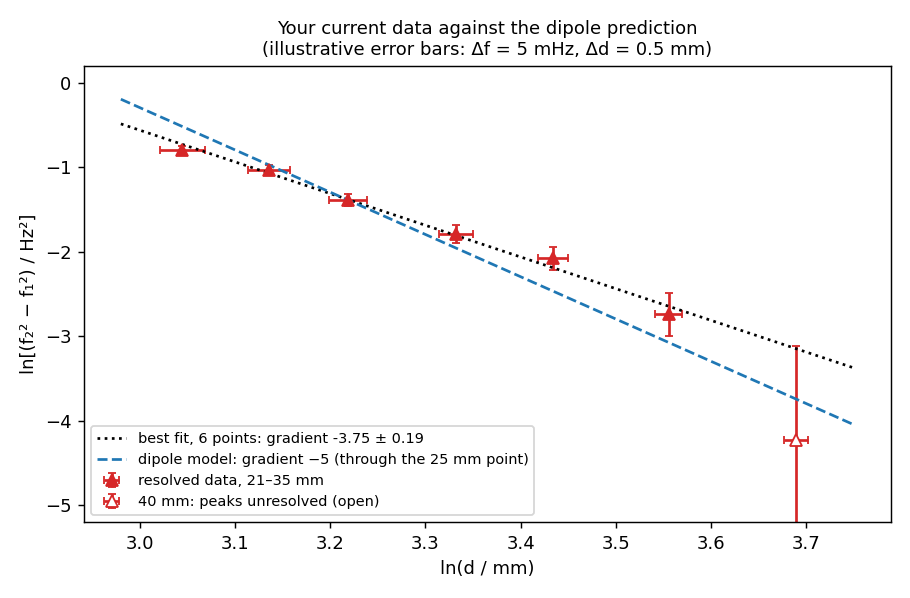
\includegraphics[width=0.78\textwidth]{F_data_vs_dipole.png}
\caption{Your current data against the dipole prediction. The 40\,mm point (open) sits far
below the resolved trend, consistent with the resolution limit of Fig.~\ref{fig:fft}, not with
new physics. Error bars are illustrative ($\Delta f=5$\,mHz, $\Delta d=0.5$\,mm) and show why
the $\ln$-transform must be weighted. \emph{Use in \S8.2/\S9.}}\label{fig:data}
\end{figure}

\begin{figure}[htbp]\centering
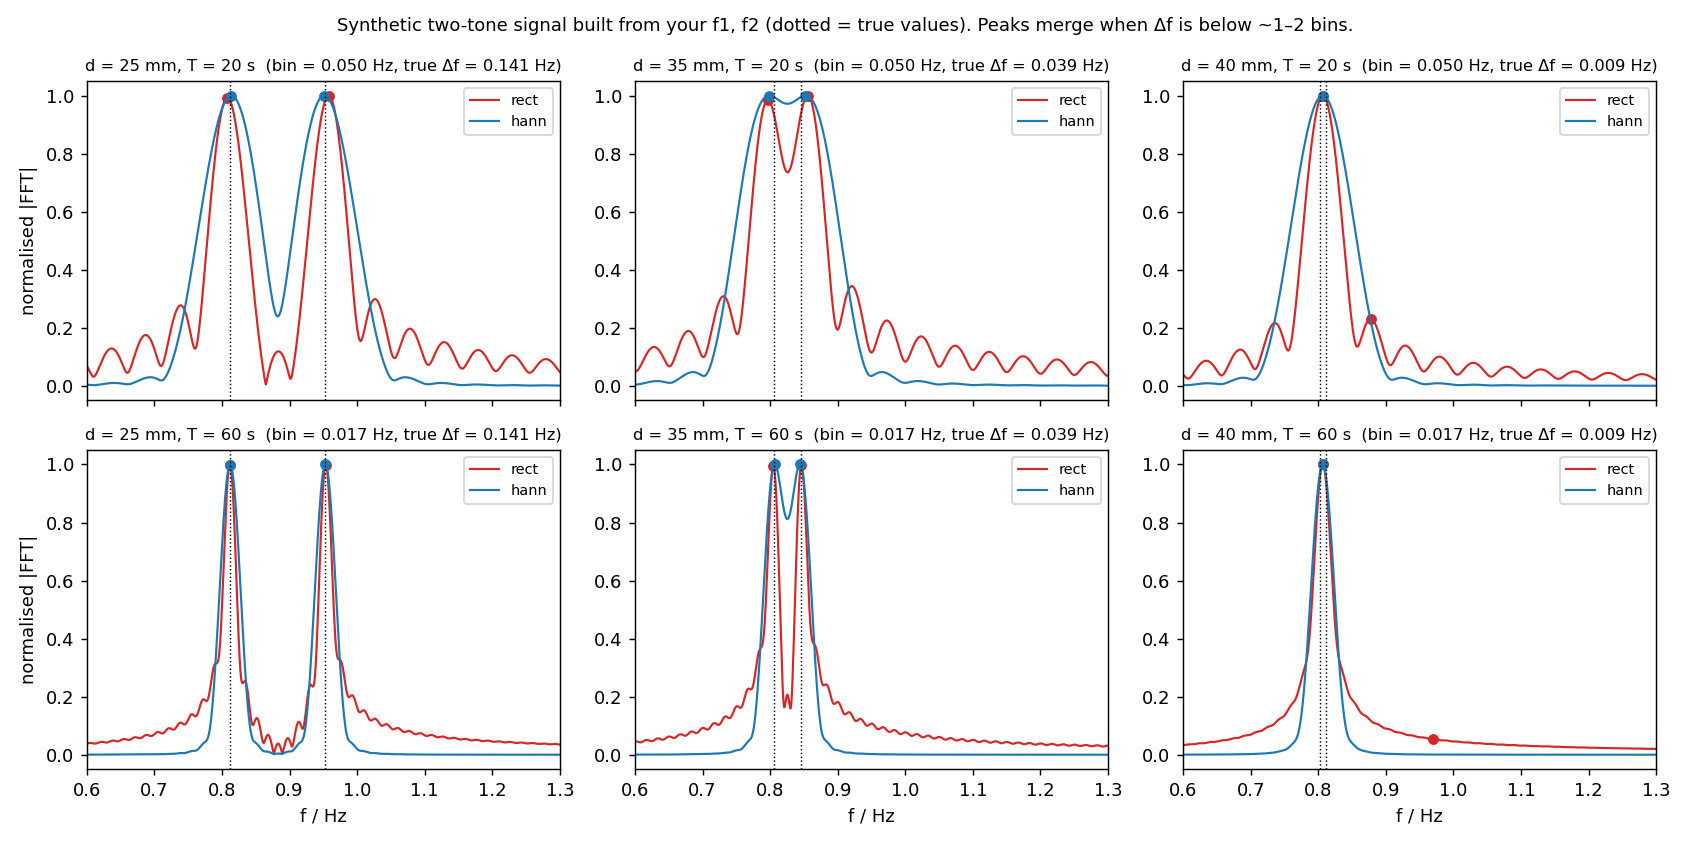
\includegraphics[width=\textwidth]{A_fft_resolution.png}
\caption{Synthetic two-tone spectra built from your $f_1,f_2$ (dotted $=$ true values) for
$T=20$ and 60\,s. Peaks merge when $f_2-f_1$ falls below $\sim$1--2 bins.
\emph{Use in \S10.1.}}\label{fig:fft}
\end{figure}

\begin{figure}[htbp]\centering
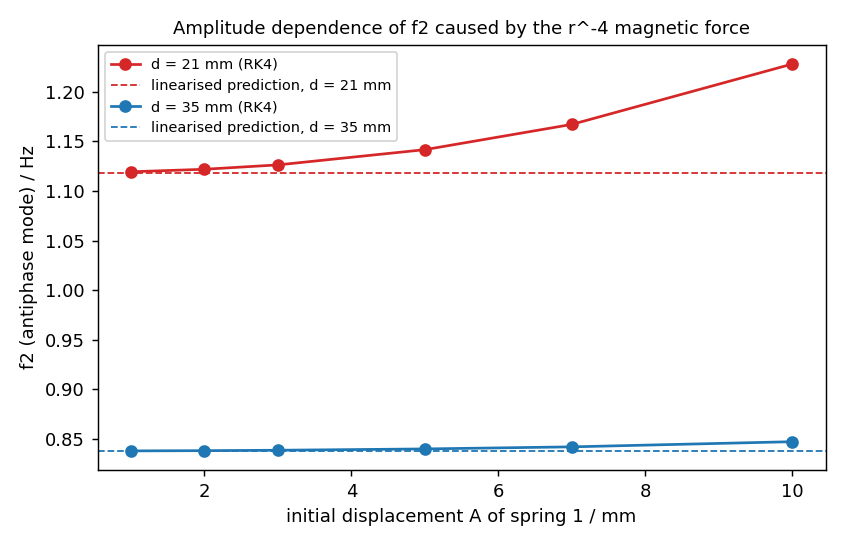
\includegraphics[width=0.62\textwidth]{B_f2_vs_amplitude.png}
\caption{RK4 simulation: $f_2$ \emph{rises} with release amplitude (hardening) relative to
the linearised prediction. \emph{Use in \S10.2/\S13.}}\label{fig:amp}
\end{figure}

\begin{figure}[htbp]\centering
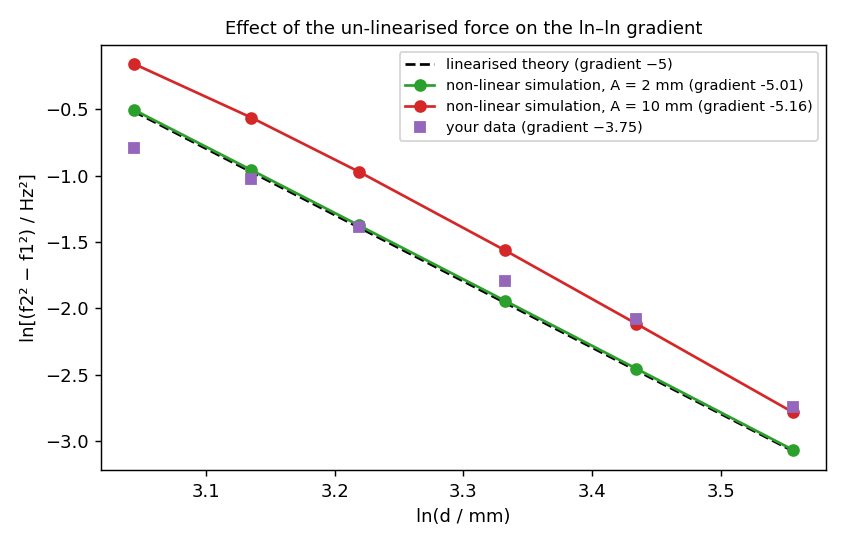
\includegraphics[width=0.62\textwidth]{B_lnln_gradient.png}
\caption{Effect of the un-linearised force on the $\ln$--$\ln$ gradient: it becomes
\emph{steeper} ($-5.16$ at $A=10$\,mm), i.e.\ the amplitude effect moves away from your
measured $-3.75$. \emph{Use in \S10.2.}}\label{fig:lnln}
\end{figure}

\begin{figure}[htbp]\centering
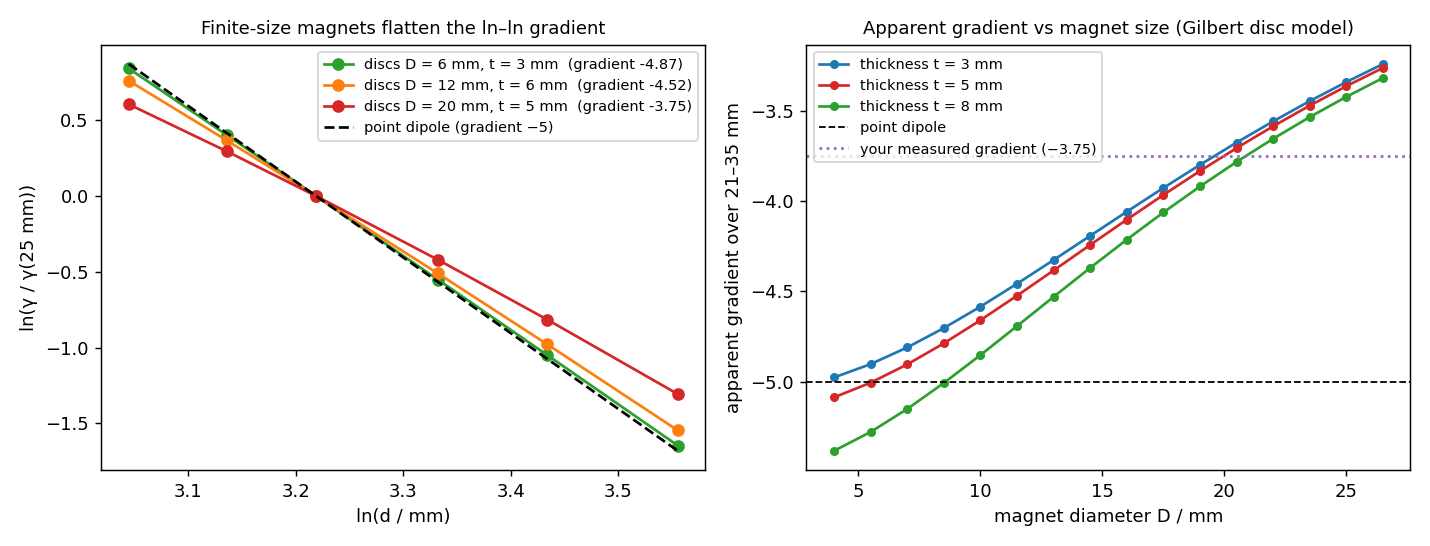
\includegraphics[width=\textwidth]{D_finite_size_gradient.png}
\caption{Finite-size (charged-disc) magnet model: the apparent gradient over 21--35\,mm
flattens as the magnet diameter grows. \emph{Use in \S10.3.}}\label{fig:finite}
\end{figure}

\begin{figure}[htbp]\centering
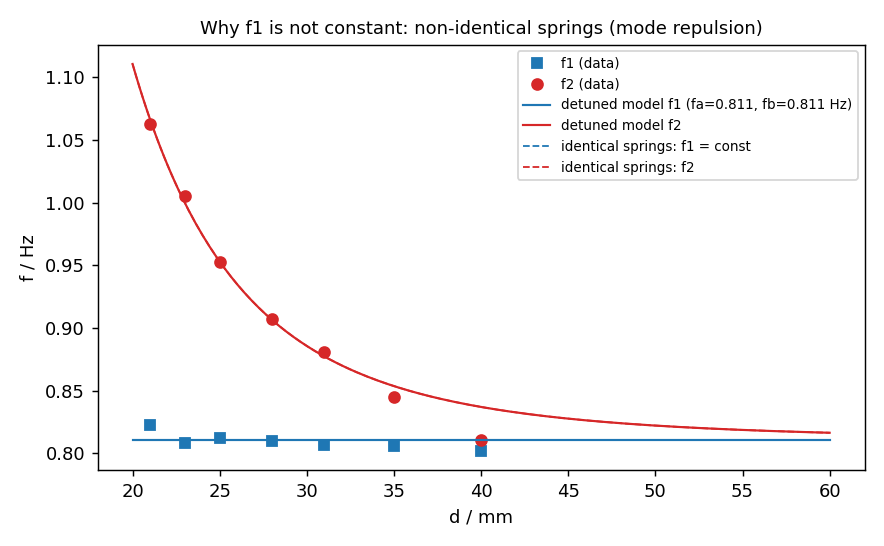
\includegraphics[width=0.62\textwidth]{E_detuning.png}
\caption{Non-identical springs: $f_1$ rises toward $\bar f$ as the coupling grows while
$f_2$ keeps increasing. \emph{Use in \S10.4.}}\label{fig:detune}
\end{figure}

\clearpage
% ===========================================================================
\section{Appendices to write}\label{sec:app}
\begin{description}[leftmargin=1.2cm,style=nextline]
\item[A] Cantilever stiffness $3EI/L^3$, effective mass $\tfrac{33}{140}\mu L$, FEM check of
lumped vs beam ($<1\,\%$); dynamic calibration $f=\tfrac1{2\pi}\sqrt{k/m}$ and why $m$ still
needs the static $k$.
\item[B] Dipole field $\to$ coaxial dipole force $F=3\muz\mum^2/(2\pi r^4)$ $\to$
$\gamma=6\muz\mum^2/(\pi d^5)$; tilt factor $3\cos\theta_1\cos\theta_2-\cos(\theta_1-\theta_2)$.
\item[C] Detuned normal modes and the limits $\kappa\to0$, $\kappa\gg\Delta$.
\item[D] Expansion of $F(d-\xi)$, $\alpha,\beta$, Landau--Lifshitz shift, comparison with RK4.
\item[E] Finite-size (charged-disc) force and apparent-gradient table.
\item[F] Uncertainty propagation: $\Delta\Y$, $\Delta\ln\Y$, $\Delta\ln d$, $\Delta d^{-5}$,
LINEST worst lines.
\item[G] Python: \texttt{analyse\_tracks.py}, \texttt{ee\_simulations.py},
\texttt{finite\_size\_magnets.py}.
\item[H] Further raw data (all windows/methods), as INTERNATIONAL Appendix~A.
\end{description}

% ===========================================================================
\section{Ready-made numbers}
\begin{notebox}
\emph{Assumed in the scripts (marked \texttt{\# ASSUMED}):} $f_s$, $\tau$, magnet size and
mass. Regenerate every number below before it enters the essay.
\begin{itemize}
\item $\ln$--$\ln$ fit, 6 points: gradient $-3.75\pm0.19$, intercept 10.68; weighted
($\Delta f=5$\,mHz): $-3.48\pm0.24$; with the 40\,mm point included: $-4.9$ (spurious).
Free power law on raw $\Y$: $n=3.5\pm0.2$.
\item Non-linear force, $A=10$\,mm: $f_2$ $+9.8\,\%$ (21\,mm), $+1.1\,\%$ (35\,mm);
gradient $-5.00\to-5.16$. $A=2$\,mm: $+0.3\,\%$, $+0.03\,\%$.
\item Finite-size discs, apparent gradient over 21--35\,mm: $D=6$\,mm $-4.87$; 10\,mm $-4.6$;
12\,mm $-4.5$; 15\,mm $-4.2$; 20\,mm $-3.75$; 25\,mm $-3.4$ ($t=3$--6\,mm changes these by $<0.1$).
\item Lumped vs beam: $\Y$ differs by 0.03\,\% ($M/\mu L=3.3$), 0.4\,\% (0.8), 1\,\% (0.4).
\item Detuned model with $n=5$: $f_a=0.793$, $f_b=0.849$\,Hz reproduces $f_1$: $0.798\to0.819$\,Hz.
\item Tilt: $\theta=0.10$\,rad at $A=10$\,mm, $L=150$\,mm; interaction weaker by 0.5--1.5\,\%.
\item Synthetic tracks, $T=40$\,s: window peak-picking $-3.3$ to $-3.5$; two-tone fit $-4.9$
(true $-4.9$).
\end{itemize}
\end{notebox}

% ===========================================================================
\section{Pitfalls (examiner's eye)}
\begin{itemize}
\item Do not present the 40\,mm point as data; present the unresolved range as a measured
limit of the method.
\item Do not claim ``$f_1$ constant'' when it drifts 2.6\,\%; explain it (\S10.4).
\item Get the \emph{sign} of every systematic effect right and say which way it moves the
gradient; the amplitude effect steepens, finite size and detuning flatten.
\item Do not copy IYPT slide figures or equations; cite the problem, derive the lumped model.
\item Every graph: error bars on both axes, best/worst lines or LINEST uncertainty, units,
gradient with uncertainty, theory line overlaid.
\item Word count: equations, tables, captions, appendices excluded -- move derivations there.
\end{itemize}

\end{document}
